\section{Frontend}

Webová aplikace je z velké části napsána ve Vue.js. Tato JavaScriptová knihovna pro tvorbu uživatelských rozhraní využívá komponentový přístup, který umožňuje rozdělit uživatelské rozhraní do logických a znovupoužitelných částí. To pomáhá udržet dobrou organizaci a architekturu projektu.

\subsection{Vlastní komponenty}
Jak již bylo zmíněno, Nuxt a Vue.js jsou založeny na znovupoužívání komponent pro zachování jednoduchosti na hlavních stránkách. Vytvořil jsem devět komponent, z nichž nejdůležitější je \textbf{\textit{TimelineComp.vue}}. Tento komponent v sobě ukrývá veškeré prvky týkající se přímo časové osy, jako jsou například CSS styly nebo ovládání osy.

Na stránce, kde se nachází časová osa, je také postranní menu vytvořené v \textbf{\textit{SidebarComp.vue}}. Obsahuje uživatelské funkce, jako je přepínání barevného režimu časové osy nebo sdílení odkazu na danou osu.

Dále existují komponenty, které se přepínají podle potřeby. Například když uživatel klikne na událost, zobrazí se \textbf{\textit{ItemInfoComp.vue}}, který poskytne informace. Pokud je však uživatel v editačním režimu, objeví se \textbf{\textit{ItemEditComp.vue}}, který umožní změnit informace o události. Podobným způsobem funguje i \textbf{\textit{InfoComp.vue}}, zobrazující informace o časové ose, a \textbf{\textit{SettingsComp.vue}}, který umožňuje upravovat hodnoty časové osy. Komponent \textbf{\textit{CreateTimeline.vue}} se zobrazí pouze tehdy, když chce uživatel vytvořit novou časovou osu, a slouží k zadání potřebných informací.

Komponent \textbf{\textit{LineCard.vue}} slouží jako šablona karty jednotlivých časových os, do níž se vkládají informace o autorovi nebo letech, které osa pokrývá.

Poslední komponent je \textbf{\textit{QuillEditor.vue}} z knihovny Quill \cite{Quill-lib}, který umožňuje uživateli používat různé textové prvky.

\newpage

\subsection{Rozdělení stránek}
V Nuxt jsou stránky definovány v adresáři \textit{pages/}, kde název .vue souboru a složky/složek, ve kterých se nachází, určuje jeho URL adresu. Názvy souborů mohou být buď statické (např. pages/about, pages/login), nebo dynamické, které pracují s proměnnými, přičemž jejich jméno je v hranatých závorkách (např. pages/[id]: pokud zadáme adresu \texttt{lines/6}, zobrazí se stránka „[id].vue“ složky lines s proměnnou 6, se kterou lze dále pracovat pomocí Vue Routeru \cite{NUXT}). Základní stránka každé složky se vždy jmenuje \textit{index.vue} a její název se nezobrazuje v URL. Nuxt také ve výchozím nastavení implementuje plně přizpůsobitelnou stránku \textit{error.vue}, na kterou jste přesměrováni, pokud nastane nějaká fatální chyba.

Strukturu mé webové stránky lze rozdělit do tří vrstev. První vrstva zahrnuje přihlášení, registraci, domovskou stránku uživatele a stránku „O projektu“. Ve druhé vrstvě se nachází „Přehled časových os“ (\textit{lines/index}), kde mohou uživatelé vyhledávat vytvořené osy, zobrazit si o nich informace, aniž by museli osu načíst, nebo vytvořit nové časové osy. Poslední, třetí vrstva obsahuje samotnou časovou osu (\textit{lines/id/index}) a podrobnosti o jednotlivých událostech (\textit{lines/id/content}).

Funkci dynamických stránek jsem ve svém projektu použil dvakrát – při výběru ID dané osy a při podrobném zobrazení údajů o události. Pokud by tedy uživatel chtěl zobrazit podrobnosti o události 17 v ose s ID 123456, výsledná URL adresa bude \texttt{/lines/123456/17}.


\begin{figure}[h]
    \centering
    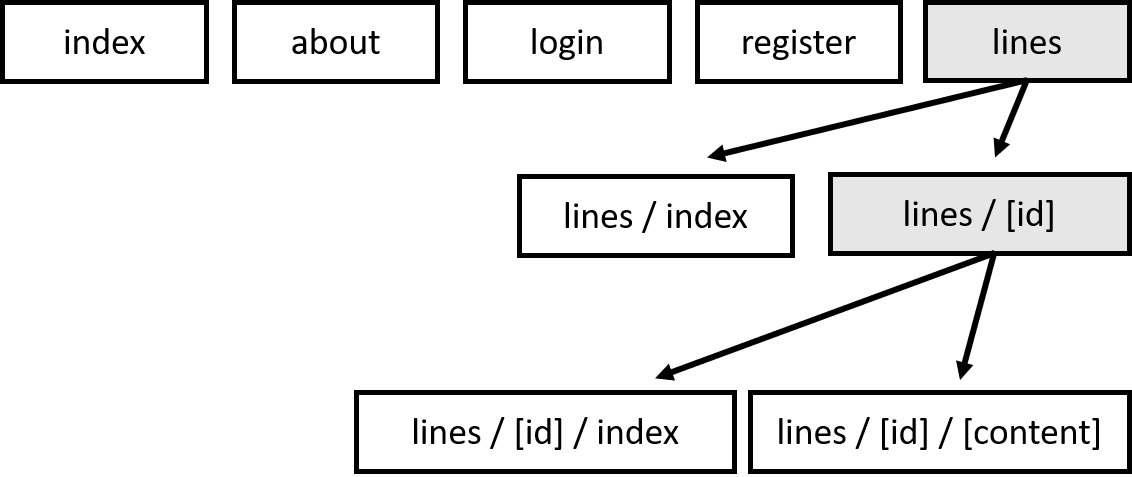
\includegraphics[width=0.8\linewidth]{Images/Tempora_pages.png}
    \caption{Rozdělení stránek ( [ ] = dynamická stránka, šedá = složka)}
    \label{fig:pages}
\end{figure}
Nuxt také používá funkci lazy-loading, která přednačítá stránky dosažitelné ze stránky aktuální pomocí speciálního odkazu NuxtLink. Tento přístup výrazně zrychluje načítání, například při rozkliknutí podrobností o události ze stránky s časovou osou.

\subsection{Moduly a knihovny}

Nuxt s Vue.js nabízí velkou škálu různých modulů, které přidávají novou funkcionalitu a rozšiřují možnosti. Jelikož jsem nikdy předtím s ekosystémem Nuxt nepracoval, na některá z těchto vylepšení jsem přicházel postupně v průběhu projektu \cite{libraries-on-EVERY-project, Nuxt3-Crash-Course}.

Jeden z nejužitečnějších modulů je NuxtUI \cite{NUXT-UI}, který přidává nejrůznější frontendové komponenty, jako jsou např. modal a toggle, ale zároveň poskytuje i vylepšené základní komponenty, například UButton, u kterého lze nastavit parametry pro ikonu, barvu či velikost. NuxtUI přidává také animovanou postranní lištu, ale tu jsem vytvořil ještě před instalací tohoto rozšíření \cite{sidebar}.

Jednou z funkcí mé aplikace je, že v zobrazení detailu můžete vidět názvy sekcí, které následují a předcházejí zobrazené sekci, což pomáhá s orientací v období. Toto zajišťuje state management framework Pinia \cite{Pinia-store}.

\subsection{Modul a komponent časové osy} \label{Komponent časové osy}

Nejdůležitější knihovna, která byla použita, je Vue Timeline Chart \cite{Vue-timeline-chart}. Hlavním důvodem, proč jsem si vybral právě tuto knihovnu, byla její flexibilita a dobře zpracovaná dokumentace. Základem této osy jsou řádky (timelineGroup) a události (timelineItem). Události mají několik údajů, jako je jméno, unikátní ID, start a end, udávané v milisekundách Unixového času (od 1. ledna 1970, 00:00:00 UTC – epoch). Základní časová osa není nijak komplikovaná, ale pokud chceme změnit její vzhled, musíme správně použít CSS a přepsat výchozí styly.

Mojí vizí bylo vytvořit dvě strany uprostřed rozdělené časovou osou, přičemž každá strana bude mít čtyři řádky s velikostí podle jejich důležitosti. Nahoře a dole bude kontext k období, dále „Hlavní skupina“, která obsahuje nadpis období, „Vedlejší skupina“, obsahující převážně autory z daného období, a nakonec „Detail skupina“, která slouží k zobrazení dalších informací, například děl daných autorů (tyto kategorie závisí na autorovi osy a může si je přizpůsobit).

\newpage

Aby osa vypadala tak, jak jsem si představoval, hrálo klíčovou roli nacházení již zavedených CSS tříd, které knihovna používá, a přepisování předem nastavených stylů pomocí syntaxe !important \cite{important-css},
viz ukázka: \ref{timestampCSS}.  
\begin{lstlisting}[style=CSS, firstnumber = 356, caption={TimelineComp.vue, Timestamps style}, label={timestampCSS}]
.timestamps {  
  transform: translateY(calc(var(--group-height) + var(--primaryGH) + var(--secondaryGH) + var(--detailGH)));
  position: absolute;
  width: 100%;
  background-color: transparent !important;
}

.timestamps:before {
  content: "";
  position: absolute;
  left: 0;
  right: 0;
  top: 50%;
  border-top: 2px solid v-bind('timelineStyles.timestamp.color');
  transform: translateY(-50%);
}

.timestamp {
  color: v-bind('timelineStyles.timestamp.color');
  position: relative;
  background-color: v-bind('timelineStyles.timestamp.backgroundColor'); 
  padding: 0 10px;
  border-left: 0px !important; 
}
\end{lstlisting}


